%%%%%%%%%%%%%%%%%%%%%%%%%%%%%%%%%%%%%%%%%
% Beamer Presentation
% LaTeX Template
% Version 1.0 (10/11/12)
%
% This template has been downloaded from:
% http://www.LaTeXTemplates.com
%
% Template Heavily modified by David Schanzenbach
%
% License:
% CC BY-NC-SA 3.0 (http://creativecommons.org/licenses/by-nc-sa/3.0/)
%
%%%%%%%%%%%%%%%%%%%%%%%%%%%%%%%%%%%%%%%%%

%----------------------------------------------------------------------------------------
%	PACKAGES AND THEMES
%----------------------------------------------------------------------------------------

%https://tex.stackexchange.com/questions/74353/what-commands-are-there-for-horizontal-spacing
%https://tex.stackexchange.com/questions/80212/controling-padding-using-the-xstring-package
%https://tex.stackexchange.com/questions/2441/how-to-add-a-forced-line-break-inside-a-table-cell
%https://en.wikibooks.org/wiki/LaTeX/Tables#The_tabularx_package
%https://tex.stackexchange.com/questions/312/correctly-typesetting-a-tilde
%https://tex.stackexchange.com/questions/34580/escape-character-in-latex
%https://tex.stackexchange.com/questions/54180/how-do-i-write-something-at-the-end-of-the-slide-in-beamer
%http://code.hammerpig.com/add-footnote-number-latex.html
%https://tex.stackexchange.com/questions/51452/reduce-spacing-in-table-of-contents-beamer
%https://www.sharelatex.com/learn/Using_colours_in_LaTeX
%http://www.math-linux.com/latex-26/article/how-to-make-a-presentation-with-latex-introduction-to-beamer
%https://stackoverflow.com/questions/3594329/semi-transparent-text-in-beamer-pdflatex
%https://www.sharelatex.com/blog/2013/08/16/beamer-series-pt3.html

%\documentclass[t]{beamer}
\documentclass[t,hyperref={pdfpagelabels=false}]{beamer}


\usepackage[T1]{fontenc}
\usepackage[utf8]{inputenc}
\usepackage{etoolbox}
\usepackage{lmodern}% http://ctan.org/pkg/lm
\usepackage{hyperref}
\usepackage{amsmath}
\usepackage{textcomp}
\usepackage{anyfontsize}
\usepackage{graphicx} % Allows including images
\usepackage{booktabs} % Allows the use of \toprule, \midrule and \bottomrule in tables
\usepackage{calc}
\usepackage{makecell}
\usepackage{xstring}
\mode<presentation> {

% The Beamer class comes with a number of default slide themes
% which change the colors and layouts of slides. Below this is a list
% of all the themes, uncomment each in turn to see what they look like.

%\usetheme{default}
%\usetheme{AnnArbor}
%\usetheme{Antibes}
%\usetheme{Bergen}
%\usetheme{Berkeley}
%\usetheme{Berlin}
%\usetheme{Boadilla}
%\usetheme{CambridgeUS}
%\usetheme{Copenhagen}
%\usetheme{Darmstadt}
%\usetheme{Dresden}
%\usetheme{Frankfurt}
%\usetheme{Goettingen}
%\usetheme{Hannover}
%\usetheme{Ilmenau}
%\usetheme{JuanLesPins}
%\usetheme{Luebeck}
%\usetheme{Madrid}
%\usetheme{Malmoe}
%\usetheme{Marburg}
%\usetheme{Montpellier}
%\usetheme{PaloAlto}
%\usetheme{Pittsburgh}
%\usetheme{Rochester}
%\usetheme{Singapore}
%\usetheme{Szeged}
%\usetheme{Warsaw}


\usetheme{ITS_CI}

% As well as themes, the Beamer class has a number of color themes
% for any slide theme. Uncomment each of these in turn to see how it
% changes the colors of your current slide theme.

%\usecolortheme{albatross}
%\usecolortheme{beaver}
%\usecolortheme{beetle}
%\usecolortheme{crane}
%\usecolortheme{dolphin}
%\usecolortheme{dove}
%\usecolortheme{fly}
%\usecolortheme{lily}
%\usecolortheme{orchid}
%\usecolortheme{rose}
%\usecolortheme{seagull}
%\usecolortheme{seahorse}
%\usecolortheme{whale}
%\usecolortheme{wolverine}

%\setbeamertemplate{footline} % To remove the footer line in all slides uncomment this line
%\setbeamertemplate{footline}[page number] % To replace the footer line in all slides with a simple slide count uncomment this line

\setbeamertemplate{navigation symbols}{} % To remove the navigation symbols from the bottom of all slides uncomment this line
}

\let\Tiny=\tiny
\definecolor{links}{HTML}{2A1B81}
\hypersetup{colorlinks,linkcolor=,urlcolor=links}

\makeatletter
\newcommand{\setlistspacing}[2]{\def\@ld{#1}\expandafter\def\csname
@list\romannumeral\@ld \endcsname{\leftmargin\csname
leftmargin\romannumeral\@ld \endcsname
              \topsep    #2
              \parsep    0\p@   \@plus\p@
              \itemsep   #2}}
\makeatother

\makeatletter
\patchcmd{\beamer@sectionintoc}{\vskip1.5em}{\vskip0.5em}{}{}
\makeatother


\newlength{\okinalen}
\setlength{\okinalen}{\widthof{'}}
\newcommand{\okina}{\hbox to.666\okinalen{\hss`\hss}}
\newcommand{\ctilde}{{\fontfamily{ptm}\selectfont\texttildelow}}

\newcommand{\trademark}{\fontsize{5}{6}\selectfont \textsuperscript{\texttrademark}}
\newcommand{\regtrademark}{\fontsize{5}{6}\selectfont \textsuperscript{\textregistered}}
\newcommand{\numlessfootnotetxt}[1]{ \let\thefootnote\relax\footnotetext{#1}}

\newcommand{\semitransp}[2][35]{\color{fg!#1}#2}
\newcommand{\btVFill}{\vskip0pt plus 1filll}
\newcommand{\ddash}{-{}-}

\newcommand{\hawaii}{Hawai{\okina}i}
\newcommand{\lustre}{Lustre{\regtrademark}}
\newcommand{\intel}{Intel{\regtrademark}}
\newcommand{\cray}{Cray{\regtrademark}}

\newcommand{\craycs}{Cray~CS300}

\newcommand{\ci}{Cyberinfrastructure}
\newcommand{\citeam}{CI--Team}

\newcommand\padfrom[2]{\StrLen{#2}[\templen]\StrGobbleLeft{#1}{\templen}#2}


\AtBeginSection[]
{
   \begin{frame}
       \frametitle{Outline}
       \tableofcontents[currentsection, hideallsubsections]
   \end{frame}
}



%\AtBeginSubsection[]
%{
%   \begin{frame}
%       \frametitle{Outline}
%       \tableofcontents[currentsection,currentsubsection]
%   \end{frame}
%}


%----------------------------------------------------------------------------------------
%	TITLE PAGE
%----------------------------------------------------------------------------------------

\title[HPC--101]{HPC--101\\Onboarding} % The short title appears at the bottom of every slide, the full title is only on the title page

\author{Gwen Jacobs Ph.D,\\Sean Cleveland Ph.D, Ron Merrill Ph.D,\\David Schanzenbach M.S.}
\institute[University of {\hawaii} -- ITS--CI] % Your institution as it will appear on the bottom of every slide, may be shorthand to save space
{
Information Technology Services \\
{\ci} \\
University of {\hawaii} \\ % Your institution for the title page
\medskip
\textbf{\url{https://www.hawaii.edu/its/ci/}}\\
\textbf{\textit{uh-hpc-help@lists.hawaii.edu}} % Your email address
}
\date{\today} % Date, can be changed to a custom date

\begin{document}

\begin{frame}
\titlepage % Print the title page as the first slide
\end{frame}

\begin{frame}
\frametitle{Outline} % Table of contents slide, comment this block out to remove it
\tableofcontents[hideallsubsections] % Throughout your presentation, if you choose to use \section{} and \subsection{} commands, these will automatically be printed on this slide as an overview of your presentation
\end{frame}

\section{Introduction}

\subsection{Parallel Computing}
\begin{frame}
	\frametitle{Parallel Computing}
	\begin{itemize}
		\item High Performance Compute
		\begin{itemize}
			\item Each separate process can send and receive data amongst other processes (MPI \& OpenMP)
			\item If processes must communicate for the overall program to proceed, high-speed networking is needed (only MPI)
		\end{itemize}
		\item High Throughput Compute
		\begin{itemize}
			\item \emph{Pleasantly Parallel} -- Processes are independent and no communication is necessary 
		\end{itemize}
	\end{itemize}
\end{frame}


\section{University of Hawai'i Cluster}

\subsection{{\craycs}}
\begin{frame}
\frametitle{{\craycs} -- History}
\begin{itemize}
 \item Initial investment of 1.8 Million by the University of {\hawaii} (UH)
 \item Delivered in October of 2014
 \item Accepted in December of 2014 
 \item Early adopter testing started in January 2015
 \item Opened for general use in April 2015
 \item March 2016, 92 new nodes added to cluster, raising total core count to 5,876 cores
 \item As of March 2016, more than 240 users have been granted access to the cluster
\end{itemize}
\end{frame}


\subsubsection{Hardware}
\begin{frame}
	\frametitle{{\craycs} -- Compute Nodes}
	\begin{itemize}
        \item All nodes are diskless with some RAM used for the Operating System
	\item 178 Standard nodes
	  \begin{itemize}
            {\footnotesize
	    \item Two 10 core {\intel} Ivy-Bridge processors (\emph{20 cores total})
	    \item 128GB of physical RAM with $\approx118$GB of useable RAM
            }
	  \end{itemize} 
          
	\item 6 Large memory nodes
	  \begin{itemize}
            {\footnotesize
	    \item Four 10 core {\intel}  Ivy-Bridge processors (\emph{40 cores total})
	    \item 1TB of physical RAM with $\approx1000$GB of useable RAM
            }
	  \end{itemize}			
        \item 1 GPU node
          \begin{itemize}
            {\footnotesize
	    \item Two 10 core {\intel} Haswell processors (\emph{20 cores total})
	    \item 128GB of physical RAM with $\approx118$GB of useable RAM
            \item 2 Nvidia Tesla K40 GPUs
            }
	  \end{itemize}
        \item 91 Owner nodes
          \begin{itemize}
            {\footnotesize
            \item 33 nodes have two 10 core {\intel} Haswell processors with 256 GB of RAM
            \item 58 nodes have two 12 core {\intel} Haswell processors with 128 GB of RAM
            }
          \end{itemize}
	\item CentOS Linux
	\end{itemize}
\end{frame}


\begin{frame}
	\frametitle{{\craycs} -- Storage}
	Two storage options are currently available on the {\craycs}
	\begin{enumerate}
		\item {\lustre}
		\item ValueStorage
	\end{enumerate}
\end{frame}


\begin{frame}
	\frametitle{{\craycs} -- Storage $\rightarrow$ {\lustre}}
	\begin{itemize}
		\item {\lustre} is a high performance parallel filesystem
		\item The {\craycs} has $\approx582$TB of storage space
		\item Shared between all compute nodes and login nodes
		\item Primarily used as scratch space for jobs (Input and Output)
		\item User do not have a usage quota (soft or hard)
		\item Certain directories are subject to a 90 day purge policy
		\item \textbf{Data is not backed up!  Users are responsible for their own data}
                \item {\lustre} utilizes RAID 6 arrays, and is fairly robust but \ldots~\\RAID is not a backup
	\end{itemize}
\end{frame}


\begin{frame}
	\frametitle{{\craycs} -- Storage $\rightarrow$ ValueStorage}
	\begin{itemize}
		\item $500$TB of scale out storage
		\item Is only available for purchase by cluster users~\\and only accessible via the login nodes
		\item Purchased in 0.5TB increments
	\end{itemize}
	\btVFill

	\begin{center}
	\textbf{ValueStorage Pricing}~\\ 
		\resizebox{0.75\textwidth}{!}{%
		\begin{tabular}{l r ||l r }
			\toprule
			\textbf{Product} & \textbf{Annual Cost}~~ & ~~\textbf{Product} & \textbf{Annual Cost}\\
	\midrule
			\midrule
			0.5TB & \$65.00~~ & ~~0.5TB + Replication  & \$130.00 \\
			\bottomrule
		\end{tabular}
		}
		~\\ \href{http://www.hawaii.edu/its/value-storage-pricing/}{More Information}
		~\\	{\footnotesize \emph{All prices are subject to change}}
	\end{center}
\end{frame}


\begin{frame}
	\frametitle{{\craycs} -- Network}
	\begin{itemize}
		\item 40Gb Infiniband inter-connects (QDR)
		\begin{itemize}
			\item High speed inter-connect between~\\compute nodes, {\lustre} storage and Login nodes
                        \item low latency ($\approx1.3\mu$s)
			\item Utilizes the \emph{fat tree network topology}
			\item[] 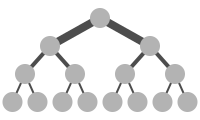
\includegraphics[width=0.20\textwidth]{images/Fat_tree_network} \\[-1ex] {\fontsize{3}{4} \selectfont Source: \url{https://en.wikipedia.org/wiki/Fat_tree} } 		
		\end{itemize}
		\item 10Gb login node internet connectivity
		\begin{itemize}
			\item Speed test from UH to CERN clocked transfer speeds up to 2$+$ Gb/s
		\end{itemize}	
	\end{itemize}
\end{frame}

\subsubsection{Layout}
\begin{frame}
	\frametitle{{\craycs} -- Layout}
	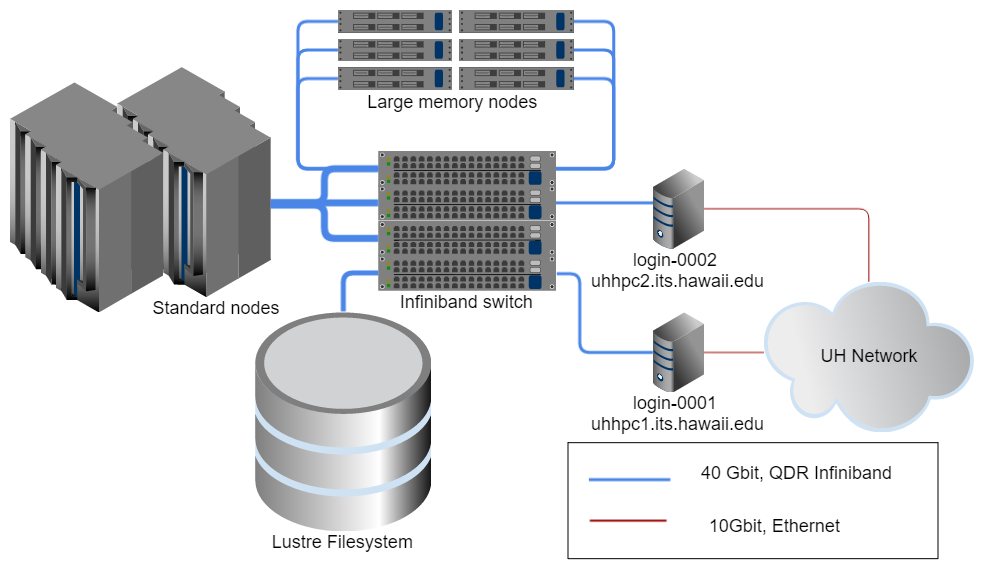
\includegraphics[width=1\textwidth]{images/layout}
\end{frame}

\section{Sustainability}
\subsection{Community Resources}
\begin{frame}
	\frametitle{Community Resources}
	\begin{itemize}
		\item The initial investment in the cluster provides resources for all faculty, staff, and students affiliated with the University of {\hawaii}
		\item All users can run on the publicly accessible partitions:\\ \emph{community.q, exclusive.q, lm.q, gpu.q, sb.q, kill.q, htc.q}
		\item For some users, the publicly available resources may not be enough~\ldots
	\end{itemize}
\end{frame}

\subsection{Ownership Models}

\subsubsection{Condo Model}
\begin{frame}
	\frametitle{Condo Model}
	\begin{itemize}
		\item The Condo model allows users to buy nodes (\emph{condos}) to incorporate into the cluster	
		\item Node owners are provided with priority access to their purchased hardware
		\item All nodes have a \emph{5 year warranty}
		\begin{itemize}
			\item Once a nodes warranty has expired, it will be removed from the cluster
		\end{itemize}
		\item Condo owners are given early access to purchased nodes
		  \begin{itemize}
                    \item Access is granted as soon as the funds land in our accounts
		    \item The 5 year warranty will not begin until newly ordered nodes are installed
		\end{itemize}
		\item Condo owners are also given the option to purchase~\\1TB of {\lustre} storage per node purchased
	\end{itemize}
\end{frame}


\subsubsection{Service Units}
\begin{frame}	
	\frametitle{Service Units}
	\begin{itemize}
	 \item In some cases, users will not require owning a node, but still need priority access
	 \item An alternative to purchasing a node, is to purchase service units (\emph{SU})
	 \item SUs come in two flavors:
		 \begin{itemize}
			 \item[--] Standard node units 
				\begin{itemize}
					\item 20 core hours, with access to 128GB of ram on a standard~node
				\end{itemize}
			 \item[--] Large memory node units
				\begin{itemize}
					\item 40 core hours, with access to 1TB of ram on a large~memory~node
				\end{itemize}
		 \end{itemize}
	 \item A minimum order totaling \$500 is required
	\end{itemize}
\end{frame}


\subsubsection{Price Card}
\begin{frame}
	\frametitle{Price Card}
	\begin{center}
	{\large \textbf{Condo Price Card}} \\
	\resizebox{\textwidth}{!}{%
		\begin{tabular}{l r ||l r}
			\toprule
			\textbf{Product} & \textbf{Cost} & \textbf{Product} & \textbf{Cost} \\
			\midrule
			\midrule
			Standard & \$6,600.00  & Standard + 2 GPUs (Nvidia{\regtrademark} K40) & \$13,600.00 \\
			\hline
			Large Memory & \$33,900.00  & 1 TB {\lustre} Storage for 5 years & \$$600.00$ \\
			\bottomrule
		\end{tabular}
		}
	\end{center}
	\smallskip
	\begin{center}
		{\large \textbf{Service Unit Price Card}}\\
		\begin{tabular}{l || c || r}
			\toprule
			\textbf{Product} & \textbf{Cost} & \textbf{Minimum Order}\\
			\midrule
			\midrule
			Standard node & \$0.50 per SU &  1,000~SU (\$500.00)\\
			Large memory node & \$2.00 per SU & 250~SU (\$500.00)\\
			\bottomrule
		\end{tabular}
		\btVFill
	{\footnotesize \emph{All prices are subject to change}}
	\end{center}
\end{frame}	



\section{Cluster Interaction}

\begin{frame}
	\frametitle{Overview -- Cluster Interaction}
	\begin{itemize}
		\item{Connecting to a cluster @ UH}
			\begin{itemize}
			\item Login to the cluster
			\item Verify user permissions
			\end{itemize}
    {\semitransp[25]{\item User directories
		\item Transferring files
		\begin{itemize}{\semitransp[25]{
			\item Globus
		}}\end{itemize}
		\item Software
		\begin{itemize}{\semitransp[25]{
			\item Modules
			\item Acquiring software
			\item Compilers
			}}
		\end{itemize}
		\item Managing user jobs
		\begin{itemize}{\semitransp[25]{
			\item Job scheduler
			\item Using SLURM
			\item Partitions			
			\item Submitting jobs (Examples)
			}}
		\end{itemize}			
		}}
	\end{itemize}
\end{frame}

\subsection{Connecting to a cluster @ UH}
\begin{frame}
	\frametitle{Connecting to a cluster @ UH}
	\begin{description}[\setlength{\leftmargini}{0pt}]
	\item[] \begin{itemize}
		\item To connect to the cluster, we utilize a client which communicates using the Secure Shell (\emph{SSH}) protocol 
		\item Linux and MacOSX, typically have a SSH client already installed
		\item Windows typically does not come with an SSH client installed
		\item Windows 10 may come pre-installed with a SSH client, but it might not be stable
		\item Suggested SSH clients for Windows include:
		\begin{itemize}
			\item \href{http://www.hawaii.edu/askus/685}{SSH Secure Shell}~(SSH 3.2.9)
			\item \href{http://www.chiark.greenend.org.uk/~sgtatham/putty/download.html}{Putty}
                        \item \href{http://mobaxterm.mobatek.net/}{MobaXterm}
		\end{itemize}
	\end{itemize}
	\item[] ~\\
	\item[] \begin{itemize}
		\item The {\craycs} has two login nodes:
		\begin{itemize}
			\item uhhpc1.its.hawaii.edu
			\item uhhpc2.its.hawaii.edu
		\end{itemize}
	\end{itemize}
	\end{description}
	{\large Let's attempt to login!}
\end{frame}


\subsubsection{Login to the {\craycs}}
\begin{frame}
\frametitle{Login to the {\craycs}}
	\begin{center}\textbf{Windows}\end{center}
	\hrule~\\
	\begin{itemize}
		\item If SSH 3.2.9 installed (Lab PCs have it installed)
		\item Open the start menu, and type ``SSH'' and you should see a program called ``SSH Secure File Terminal Client''
		\item Click ``Quick Connect'' and enter the following information:
			\begin{itemize}
			\item[] \textbf{Host Name:} uhhpc1.its.hawaii.edu --OR-- uhhpc2.its.hawaii.edu
			\item[] \textbf{User Name:} Your UH User name e.g., user99
			\item[] \textbf{Port:} 22
			\end{itemize}
		\item Press ``Connect''
		\item Enter your UH user password when prompted and press the return key
	\end{itemize}
\end{frame}


\begin{frame}
\frametitle{Login to the {\craycs}}
	\begin{center}\textbf{Mac \& Linux}\end{center}
	\hrule~\\
	\begin{itemize}
		\item Open a terminal window
		\item Enter one of the following:
		\begin{itemize}
			\item ssh $<$UH User name$>$@uhhpc1.its.hawaii.edu
			\item ssh $<$UH User name$>$@uhhpc2.its.hawaii.edu
			\item \textbf{Example:} ssh user99@uhhpc1.its.hawaii.edu
		\end{itemize}
		\item Enter your UH user password when prompted and press the return key
	\end{itemize}
\end{frame}


\begin{frame}
\frametitle{On Initial Login~\ldots}
	Validate that all system permissions are correct for your user~\\
	\begin{enumerate}
		\item Test that you can list files in your home: `\texttt{ls -la}'    
		\item Test making a file in your home: `\texttt{touch test.txt}'    
		\item Go into \ctilde{}/lus: `\texttt{cd \ctilde{}/lus/}'  
		\item Test making a file in your lus directory: `\texttt{touch test.txt}'   
		\item Go into \ctilde{}/apps:  `\texttt{cd \ctilde{}/apps/}'     
		\item Test making a file in your apps directory: `\texttt{touch test.txt}'   
	\end{enumerate}
	\begin{alertblock}{Result}
		\begin{center}Did you get any errors?  Let us know if you did\end{center}
	\end{alertblock}
	\btVFill
	
	\small Notes:
		\begin{itemize}\tiny
		\item On login you are placed in /home/$<$username$>$/
		\item By default, \ctilde{} is equivalent to /home/$<$username$>$/
		\end{itemize}
\end{frame}


\begin{frame}
	\frametitle{Overview -- Cluster Interaction}
	\begin{itemize}
		\item {\semitransp[25]{Connecting to a cluster @ UH}}
			\begin{itemize}{\semitransp[25]{
			\item Login to the cluster
			\item Verify user permissions
			}}
			\end{itemize}
    \item User directories
		{\semitransp[25]{\item Transferring files
		\begin{itemize}{\semitransp[25]{
			\item Globus
		}}\end{itemize}
		\item Software
		\begin{itemize}{\semitransp[25]{
			\item Modules
			\item Acquiring software
			\item Compilers
			}}
		\end{itemize}
		\item Managing user jobs
		\begin{itemize}{\semitransp[25]{
			\item Job scheduler
			\item Using SLURM
			\item Partitions			
			\item Submitting jobs (Examples)
			}}
		\end{itemize}			
		}}
	\end{itemize}
\end{frame}

\subsection{User Directories}
\begin{frame}[fragile]
\frametitle{User Directories}
\begin{block}{Home}
\begin{semiverbatim}\tiny \texttt
[user99@login \ctilde]\$ ls -l 
total 0
lrwxrwxrwx 1 user99 user99 23 Jan 15 20:38 \textcolor{teal}{apps} -> /lus/scratch/usr/user99
lrwxrwxrwx 1 user99 user99 19 Jan 15 20:38 \textcolor{teal}{lus} -> /lus/scratch/user99
lrwxrwxrwx 1 root   root   37 Jan 15 20:41 \colorbox{black}{\textcolor{red}{purge}} -> /lus/scratch/log/purge/current/user99
\end{semiverbatim}
\end{block}
	\begin{itemize}\footnotesize
		\item \ctilde{}/ is not on the {\lustre} filesystem and \textbf{should not be used for job data!}
		\item \ctilde{}/lus/ is a symlink to the {\lustre} scratch
		\begin{itemize}\tiny
			\item This is where all your job data files should live
			\item Items in this directory \emph{\textbf{are}} subject to our 90 day purge policy
		\end{itemize}
		\item \ctilde{}/apps/ is a symlink to where programs should be stored
		\begin{itemize}\tiny
			\item Items in this directory \emph{\textbf{are not}} subject to our 90 day purge policy
			\item Directory is monitored for abuse
		\end{itemize}
		\item \ctilde{}/purge/ is typically a dead symlink
		\begin{itemize}\tiny
			\item Symlink becomes active if the user has files that are part of the next automatic purge
			\item When \ctilde{}/purge/ is active, the directory containing two files -- \emph{purge\_list.txt} \& \emph{totals.txt}
			\item An email is sent to users if they have files that will be purged
			\item Email notification is sent out 14 days before the purge takes place
		\end{itemize}
	\end{itemize}
\end{frame}


\begin{frame}[fragile]
\frametitle{User Directories}
\begin{block}{Filesystems}
\begin{semiverbatim}\tiny \texttt
[user99@login \ctilde]\$ df -h
Filesystem                                  Size  Used Avail Use% Mounted on
10.10.0.3:/ha_cluster/home                  1.8T  888G  851G  52% /home
10.12.0.51@o2ib:10.12.0.52@o2ib:/scratch    582T  429T  125T  78% /lus/scratch
\end{semiverbatim}
\end{block}
	\begin{itemize}\footnotesize
		\item /home/$<$username$>$ exists on a NFS mounted filesystem
		\begin{itemize}\tiny
			\item Only has 1.8TB of useable space
			\item Using all this space may cause problems for the entire cluster
			\item Not a high performance filesystem and small in size
		\end{itemize}
		\item /lus/scratch/ is the {\lustre} filesystem
		\begin{itemize}\tiny
			\item Has 582TB of useable space
			\item \ctilde{}/apps/, \ctilde{}/lus/, and \ctilde{}/purge/ all point to directories on this filesystem
			\item High performance and a lot more space for users to use
			\item No hard or soft quotas are in place
			\item Utilization is managed through the 90 day purge policy
		\end{itemize}
	\end{itemize}
\end{frame}


\begin{frame}
	\frametitle{Overview -- Cluster Interaction}
	\begin{itemize}
		\item {\semitransp[25]{Connecting to a cluster @ UH}}
			\begin{itemize}{\semitransp[25]{
			\item Login to the cluster
			\item Verify user permissions
			}}
			\end{itemize}
    {\semitransp[25]{\item User directories}}
		\item Transferring files
		\begin{itemize}
			\item Globus
		\end{itemize}
		{\semitransp[25]{
		\item Software
		\begin{itemize}{\semitransp[25]{
			\item Modules
			\item Acquiring software
			\item Compilers
			}}
		\end{itemize}
		\item Managing user jobs
		\begin{itemize}{\semitransp[25]{
			\item Job scheduler
			\item Using SLURM
			\item Partitions			
			\item Submitting jobs (Examples)
			}}
		\end{itemize}			
		}}
	\end{itemize}
\end{frame}


\subsection{Transferring Files}
\begin{frame}
	\frametitle{Available File Transfer Protocols}
	\begin{itemize}
		\item The cluster has the following options for transferring files:
		\begin{itemize}
			\item[--] scp (RCP$+$SSH protocol)
			\item[--] rsync (rsync protocol with SSH transport)
			\item[--] SFTP (SSH FTP protocol) -- Filezilla, Cyberduck
			\item[--] \href{https://www.globus.org/}{Globus} (Grid FTP protocol)
		\end{itemize}
		\item All options are widely used, and have clients that can be found for on most major operating systems
%               \item Please see the the CI website for links to several different clients?                 
	\end{itemize}
	\btVFill
	\begin{center}
		SFTP, scp, and rsync are fairly common on Linux systems,~\\but Globus is not as common~\ldots
	\end{center}
	
\end{frame}


\subsection{Globus}
\begin{frame}
	\frametitle{Globus}
	\begin{block}{What is Globus?}\footnotesize
	The Globus transfer service provides high-performance, secure, file transfer and synchronization between endpoints.~\\~\\
	Globus handles all the difficult aspects of data transfer, allowing application users to easily start and manage transfers between endpoints, while automatically tuning parameters to maximize bandwidth usage, managing security configurations, providing automatic fault recovery, and notifying users of completion and problems. 
	\end{block}
	\begin{definition}\tiny
	An \textbf{\emph{endpoint}} is one of the two file transfer locations -- either the source or the destination -- between which files can move.~\\Once a resource (such as a server, cluster, storage system, laptop, or other system) is defined as an endpoint, it will be available to authorized users who can transfer files to or from this endpoint.
	\end{definition}
\numlessfootnotetxt{\tiny \url{https://www.globus.org/file-transfer}}
\end{frame}

\begin{frame}
	\frametitle{Globus}\footnotesize
\begin{block}{How do I get Globus?}
To utilize Globus, follow the following steps:
\begin{itemize}\tiny
\item Register for a Globus Online account -- \url{https://www.globusonline.org/signup}
\item Sign in to Globus Online (using your Globus Online username and password) -- \url{https://www.globusonline.org/signin}
\item Select ‘Start Transfer’ under ‘File Transfer’, or from the drop down menu in the top bar
\item You can view the list of available endpoints by clicking the button on the ‘Endpoint’ drop down box
\begin{itemize}\tiny
 \item Each of the login nodes is also an endpoint: \textbf{\emph{hawaii\#UHHPC1}} \& \textbf{\emph{hawaii\#UHHPC2}}
\end{itemize}
\item Once you select an endpoint, a login window will pop up. You can access the UHHPC endpoints by simply using your UH username and password. Enter your UH accounts username in the ‘Username’ field and UH accounts password in the ‘Password’ field and click ‘Authenticate’. 
\item You will see a listing of the contents of your home directory on the UH HPC. Double click on a directory to view its contents
\item Select a file or directory and click on the highlighted ‘arrow button’ to initiate the transfer
\end{itemize}
\end{block}
~\\
These instructions can also be found on the {\ci} website:~\\
{\footnotesize \href{http://www.hawaii.edu/its/ci/hpc-resources/hpc-tutorials/globus-quick-start-guide/}{http://www.hawaii.edu/its/ci/hpc-resources/hpc-tutorials/globus-quick-start-guide/}}
\end{frame}


\begin{frame}
	\frametitle{Globus}
        \begin{itemize}
          \item In order to transfer data from the {\craycs} to your personal computer, a client called the Globus Connect Personal (\url{https://www.globus.org/globus-connect-personal}) needs to be installed
          \item The Globus Connect Personal, turns your personal computer into a private endpoint that is only useable with your personal Globus Online account.
          \item If you want to install Globus on your own server, Globus Connect (\url{https://www.globus.org/globus-connect-server}) is required
            \item If issues arise while trying to install Globus Connect or Globus Connect Personal,  please contact us and we will be more than happy to help
\end{itemize} 
\end{frame}

\begin{frame}
	\frametitle{Overview -- Cluster Interaction}
	\begin{itemize}
		\item {\semitransp[25]{Connecting to a cluster @ UH}}
			\begin{itemize}{\semitransp[25]{
			\item Login to the cluster
			\item Verify user permissions
			}}
			\end{itemize}
   {\semitransp[25]{ \item User directories
		\item Transferring files
		\begin{itemize}{\semitransp[25]{
			\item Globus
		}}\end{itemize}
		}}
		\item Software
		\begin{itemize}
			\item Modules
			\item Acquiring software
			\item Compilers
		\end{itemize}
		{\semitransp[25]{
		\item Managing user jobs
		\begin{itemize}{\semitransp[25]{
			\item Job scheduler
			\item Using SLURM
			\item Partitions
			\item Submitting jobs (Examples)
			}}
		\end{itemize}			
		}}
	\end{itemize}
\end{frame}


\subsection{Software}
\begin{frame}
	\frametitle{Modules}
	\begin{block}{Modules}\tiny
	A tool to help users manage their Unix or Linux shell environment, by allowing groups of related environment-variable settings to be made or removed dynamically.\footnotemark
	
	\end{block}
	\begin{itemize}
		\item We globally install frequently requested software packages and create modules for all users to access
		\item Access to modules is via the \textbf{module} command
		\begin{itemize}\footnotesize
			\item `module avail' -- list installed modules
			\item `module show $<$module name$>$' -- Show what actions a module performs
			\item `module load $<$module name$>$' -- Loads the named module
			\item `module purge' -- Unload all loaded modules
		\end{itemize}
		\item Installing software in your \ctilde{}/apps directory is suggested to prevent us from being a bottleneck
	\end{itemize}
	\footnotetext[1]{\tiny \url{https://en.wikipedia.org/wiki/Environment_Modules_(software)}}
\end{frame}


\begin{frame}
	\frametitle{Acquiring Software -- Binaries and/or Source}
	\begin{itemize}
		\item	You can transfer software source, binaries or scripts into your \ctilde{}/apps directory on the {\craycs}
		\begin{itemize}
			\item Binaries compiled as x86\_64 (64-bit) for CentOS 6.5 or RHEL6.5 should work
		\end{itemize}
		\item You may also download tar or zipped software/source code directly from the login nodes using tools like \textbf{wget} \& \textbf{curl}
		\item You may also clone source repositories using the correct software revision tool: \textbf{git}, \textbf{svn}, \textbf{hg}, \textbf{cvs}, etc.
	\end{itemize}
\end{frame}


\begin{frame}
\frametitle{Compilers}
	\begin{itemize}
		\item We have the {\intel}, GNU (gcc, g$++$), {\cray} \& PGI{\regtrademark} compilers
		\item Compiling must take place on a compute node
		\begin{itemize}
			\item Interactive sessions are useful for compiling software
			\item Sandbox nodes mirror the environment the compute nodes provide and are ideal for compilation
			\item Login nodes \textbf{do not} load all the software and libraries found on the compute nodes
		\end{itemize}
		\item {\intel} compilers are recommended for best performance
		\begin{itemize}
			\item {\intel} 2013 compilers:
			\begin{itemize}
				\item module load intel/ics -- Loads {\intel} compilers: {\tiny \textbf{icc}, \textbf{ifort}, \textbf{icpc}}
				\item module load intel/impi -- Loads {\intel} MPI wrapper: {\tiny\textbf{mpiicc}, \textbf{mpiifort}, \textbf{mpiicpc}}
			\end{itemize}
			\item {\intel} 2016 compilers:
			\begin{itemize}
				\item We have 2 floating seats for {\intel} 2016 compiler
				\item intel\_2016/ics 
				\item intel\_2016/impi 
			\end{itemize}
		\end{itemize}			
	\end{itemize}
\end{frame}


\begin{frame}
	\frametitle{Overview -- Cluster Interaction}
	\begin{itemize}
		\item {\semitransp[25]{Connecting to a cluster @ UH}}
			\begin{itemize}{\semitransp[25]{
			\item Login to the cluster
			\item Verify user permissions
			}}
			\end{itemize}
   {\semitransp[25]{ \item User directories
		\item Transferring files
		\begin{itemize}{\semitransp[25]{
			\item Globus
		}}\end{itemize}
		\item Software
		\begin{itemize}{\semitransp[25]{
			\item Modules
			\item Acquiring software
			\item Compilers
			}}
		\end{itemize}
		}}
		\item Managing user jobs
		\begin{itemize}
			\item Job scheduler
			\item Using SLURM
			\item Partitions
			\item Submitting jobs (Examples)
		\end{itemize}		
	\end{itemize}
\end{frame}


\subsection{Managing User Jobs}
\begin{frame}
\frametitle{Managing User Jobs}
User jobs all come in different shapes and sizes:  
\begin{itemize}\footnotesize
	\item Require multiple nodes working in concert towards a common goal (MPI)
	\item Require a single node, in which they use multiple threads~\\work together (OpenMP, pthreads)
	\item Require a lot of cores to process a lot of data in an identical manner,~\\yet none of the inputs have dependencies on another (HTC)
\end{itemize}
\bigskip
The {\craycs} is capable of handling many different types of jobs, but with so many users in a multi-user environment, how do we impose order on this chaos?
\btVFill
\begin{center}This looks like a job for a \textbf{\emph{job scheduler}}!\end{center}
\end{frame}

\begin{frame}
  \frametitle{Job Schedulers}
  \begin{block}{Purpose}To control and prioritize the execution order of unrelated jobs\end{block}
	Basic features expected of a job scheduler:
	\begin{itemize}\footnotesize
        \item Provides a user interface for users to request resources and monitor work 
        \item Allocates access to resources for the requested duration of time
	\item Starts, monitors and terminates work on allocated resources
	\item Arbitrates contention for resources by managing queues of pending work
	\end{itemize}
	\bigskip
        The {\craycs} uses the \textbf{S}imple \textbf{L}inux \textbf{U}tility for \textbf{R}esource \textbf{M}anagement~\\ or simply known as the \emph{SLURM scheduler}
	\numlessfootnotetxt{\tiny \url{https://en.wikipedia.org/wiki/Slurm_Workload_Manager}}
	\numlessfootnotetxt{\tiny \url{http://slurm.schedmd.com/slurm.html}}
\end{frame}

\subsection{SLURM}
\begin{frame}
\frametitle{SLURM}
\begin{block}{How are jobs scheduled?}
User submitted jobs are assigned a priority using a fairshare algorithm.\\
Factors such as the following are all used to assign a priority to a given job: 
\begin{itemize}
\item Runtime
\item Resource usage request
\item Age of job
\item Amount of core hours a user has used in recent history
\end{itemize}

\end{block}
\end{frame}

\begin{frame}
\frametitle{SLURM commands}\footnotesize
SLURM has a series of commands, each of which allow users to interact with the job scheduler
\begin{itemize}\tiny
	\item \emph{\textbf{srun}} --  Used to submit a job for execution or initiate job steps in real time
	\item \emph{\textbf{sbatch}} -- Used to submit a job script for later execution. The script could contain one or more srun commands
	\item \emph{\textbf{squeue}} -- Reports the state of jobs or job steps
	\item \emph{\textbf{scancel}} -- Used to cancel a pending or running job or job step. It can also be used to send an arbitrary signal to all processes associated with a running job or job step
	\item \emph{\textbf{sinfo}} -- Reports the state of partitions and nodes managed by Slurm. It has a wide variety of filtering, sorting, and formatting options
	\item \emph{\textbf{sacct}} -- Used to report job or job step accounting information about active or completed jobs
	\item \emph{\textbf{scontrol}} -- The administrative tool used to view and/or modify Slurm state. Note that many scontrol commands can only be executed as user root
\end{itemize}
\begin{itemize}
	\item[--] Examples usage of the SLURM commands can be seen on schedmd's \href{http://slurm.schedmd.com/quickstart.html}{quickstart}
	\item[--] Each command should have a `man' page, or displays help when the -h flag is used
\end{itemize}
\numlessfootnotetxt{\tiny \url{http://slurm.schedmd.com/quickstart.html}}
\end{frame}


\subsection{SLURM Partitions}
\begin{frame}
\footnotesize
\frametitle{Partitions}
\begin{block}{What is a partition?}\footnotesize
A partition can be thought of as a group of nodes/resources divided into possibly overlapping sets.  Each partition can be considered as a job queue, each of which has an assortment of constraints such as job size limit, job time limit, users permitted to use it, etc. Priority-ordered jobs are allocated nodes within a partition until the resources (nodes, processors, memory, etc.) within that partition are exhausted.\footnotemark
\end{block}
\begin{itemize}
	\item The {\craycs} currently has seven public partitions:~\\\textbf{community.q}, \textbf{exclusive.q}, \textbf{lm.q}, \textbf{gpu.q}, \textbf{sb.q}, \textbf{kill.q}, \textbf{htc.q}
	\item Jobs submitted to kill.q and htc.q can be preempted by jobs in other partitions
\end{itemize}
\footnotetext[2]{\tiny \url{http://slurm.schedmd.com/quickstart.html}}
\end{frame}

\begin{frame}
\frametitle{Partitions}
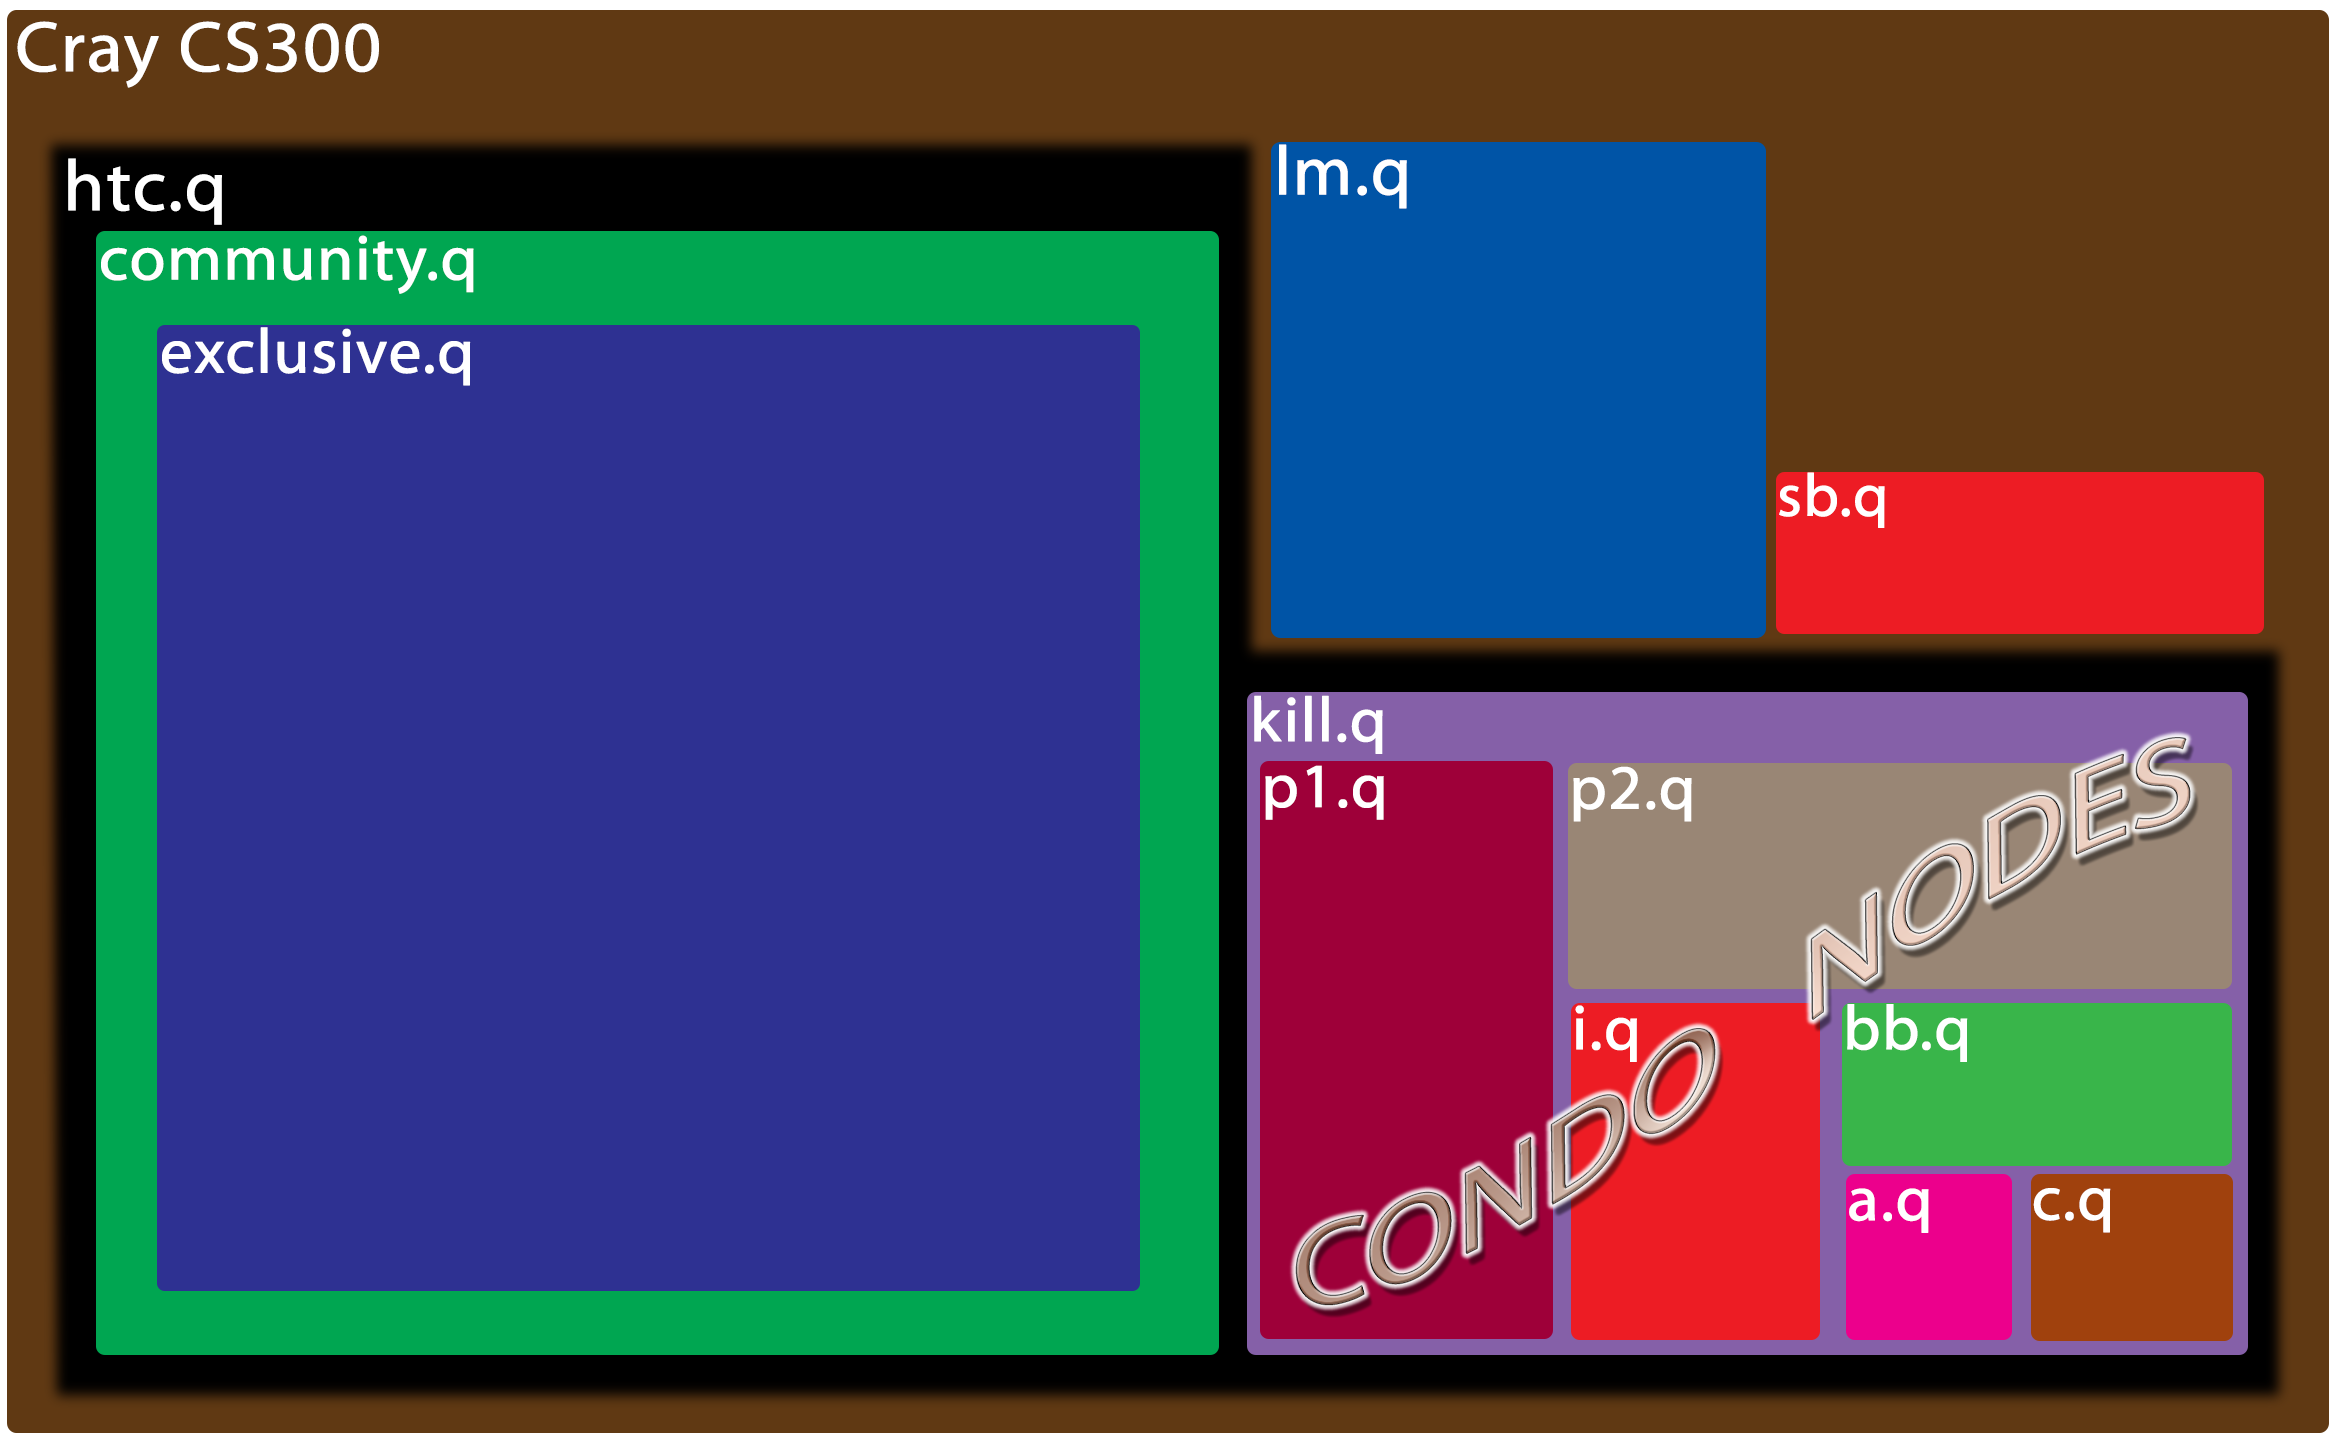
\includegraphics[width=0.95\textwidth]{images/partitions}
\end{frame}

\begin{frame}
\frametitle{Partition Details}
\resizebox{0.95\textwidth}{!}{%
\begin{tabular}{l || c || c || c || c || c || c}
\toprule                                                                    
\textbf{Partition} & \textbf{Time} & \textbf{Nodes per job} & \textbf{Priority} & \textbf{Shared} & \textbf{Preempt Mode} & \textbf{Memory per CPU (MB)} \\
%\toprule                                                                    
%\toprule                                                                    
\midrule
\midrule
community.q & \begin{tabular}{l r} \textbf{Default:} & 0-00:10:00~\\ \textbf{Max:} & 3-00:00:00\end{tabular} & \begin{tabular}{c c} \textbf{Min:} & \padfrom{\ \ \ }{1}~\\ \textbf{Max:} & \padfrom{\ \ \ }{20}\end{tabular} & 10 & NO & OFF & \begin{tabular}{l c}\textbf{Default:} & \padfrom{\ \ \ \ \ \ \ }{3250}~\\ \textbf{Max:} & \padfrom{\ \ \ \ \ \ \ \ }{$\infty$}\end{tabular}\\
\hline
\hline
exclusive.q & \begin{tabular}{l r}\textbf{Default:} & 0-00:10:00~\\ \textbf{Max:} & 3-00:00:00\end{tabular} &  \begin{tabular}{c  c}\textbf{Min:}& \padfrom{\ \ \ }{1}~\\ \textbf{Max:}&\padfrom{\ \ \ }{20}\end{tabular} & 10 & EXCLUSIVE & OFF & \begin{tabular}{l c}\textbf{Default:} & \padfrom{\ \ \ \ \ \ \ \ }{$\infty$}~\\ \textbf{Max:} & \padfrom{\ \ \ \ \ \ \ \ }{$\infty$}\end{tabular}\\
\hline
\hline
gpu.q & \begin{tabular}{l r} \textbf{Default:} & 0-00:10:00~\\ \textbf{Max:} & 3-00:00:00\end{tabular} & \begin{tabular}{c c} \textbf{Min:} & \padfrom{\ \ \ }{1}~\\ \textbf{Max:} & \padfrom{\ \ \ }{1}\end{tabular} & 10 & NO & OFF & \begin{tabular}{l c}\textbf{Default:} & \padfrom{\ \ \ \ \ \ \ }{3250}~\\ \textbf{Max:} & \padfrom{\ \ \ \ \ \ \ \ }{$\infty$}\end{tabular}\\
\hline
\hline
kill.q & \begin{tabular}{l r}\textbf{Default:} & 0-00:10:00~\\ \textbf{Max:} & 3-00:00:00\end{tabular} &  \begin{tabular}{c  c}\textbf{Min:} & \padfrom{\ \ \ }{1}~\\ \textbf{Max:} &\padfrom{\ \ \ }{12}\end{tabular} & 10 & NO & REQUEUE & \begin{tabular}{l c}\textbf{Default:} & \padfrom{\ \ \ \ \ \ \ }{3250}~\\ \textbf{Max:} & \padfrom{\ \ \ \ \ \ \ \ }{$\infty$}\end{tabular}\\
\hline
\hline
htc.q & \begin{tabular}{l r}\textbf{Default:} & 0-00:10:00~\\ \textbf{Max:} & 3-00:00:00\end{tabular} &  \begin{tabular}{c  c}\textbf{Min:} & \padfrom{\ \ \ }{1}~\\ \textbf{Max:} &\padfrom{\ \ \ }{1}\end{tabular} & 1 & NO & REQUEUE & \begin{tabular}{l c}\textbf{Default:} & \padfrom{\ \ \ \ \ \ \ }{3250}~\\ \textbf{Max:} & \padfrom{\ \ \ \ \ \ \ \ }{$\infty$}\end{tabular}\\
\hline
\hline
lm.q & \begin{tabular}{l r}\textbf{Default:} & 0-00:10:00~\\ \textbf{Max:} & 3-00:00:00\end{tabular} &  \begin{tabular}{c  c}\textbf{Min:} & \padfrom{\ \ \ }{1}~\\ \textbf{Max:} &\padfrom{\ \ \ }{1}\end{tabular} & 10 & NO & OFF & \begin{tabular}{l c}\textbf{Default:} & \padfrom{\ \ \ \ \ \ \ \ }{$\infty$}~\\ \textbf{Max:} & \padfrom{\ \ \ \ \ \ \ \ }{$\infty$}\end{tabular}\\
\hline
\hline
sb.q & \begin{tabular}{l r}\textbf{Default:} & 0-00:05:00~\\ \textbf{Max:} & 0-01:00:00\end{tabular} &  \begin{tabular}{c  c}\textbf{Min:} & \padfrom{\ \ \ }{1}~\\ \textbf{Max:} &\padfrom{\ \ \ }{2}\end{tabular} & 10 & NO & OFF & \begin{tabular}{l c}\textbf{Default:} & \padfrom{\ \ \ \ \ \ \ }{3250}~\\ \textbf{Max:} & \padfrom{\ \ \ \ \ \ \ \ }{$\infty$}\end{tabular}\\
\bottomrule 
\end{tabular}   
}
\\
\bigskip
Partition details also available on the \href{http://www.hawaii.edu/its/ci/hpc-resources/slurm-partitions/}{{\ci} website} or by using the following command:
\\
\texttt{$[$login \ctilde$]$\$ scontrol show partition $<$partition name$>$}
\end{frame}

\subsection{Interactive Job -- srun}
\frametitle{SLURM Job Scripts}
\begin{frame}
\frametitle{Interactive Job with SLURM}
	\begin{block}{Interactive session}\tiny
	$[$login \ctilde$]$\$ srun \ddash{}immediate \ddash{}partition sb.q \ddash{}nodes 1 \ddash{}cpus-per-task 1 \ddash{}tasks-per-node 1 \ddash{}time 0-01:00:00 \ddash{}pty /bin/bash
          ~\\
          ~\\
          \hrule
          ~\\
	$[$login \ctilde$]$\$ srun -I -p sb.q -N 1 -c 1 -n 1 -t 0-01:00:00 \ddash{}pty /bin/bash

	\end{block}
\end{frame}



\subsection{MPI Batch Job Example Script}
\begin{frame}[fragile]
\frametitle{SLURM sbatch -- Submission Script File (MPI Job)}
\begin{semiverbatim}\tiny
[login lus]\$ cat mpi.slurm

\#!/bin/bash
\#SBATCH \ddash{}job-name=MPI\_example
\#SBATCH \ddash{}partition=exclusive.q
\#\# 3 day max run time for community.q, kill.q, exclusive.q, and htc.q.  1 Hour max run time for sb.q
\#SBATCH \ddash{}time=3-00:00:00 ## time format is DD-HH:MM:SS
\#\# task-per-node x cpus-per-task should not typically exceed core count on an individual node 
\#SBATCH \ddash{}nodes=4
\#SBATCH \ddash{}tasks-per-node=20
\#SBATCH \ddash{}cpus-per-task=1
\#SBATCH \ddash{}error=hello-\%A.err \#\# \%A - filled with jobid
\#SBATCH \ddash{}output=hello-\%A.out \#\# \%A - filled with jobid
\#\# Useful for remote notification
\#SBATCH \ddash{}mail-type=BEGIN,END,FAIL,REQUEUE,TIME\_LIMIT\_80
\#SBATCH \ddash{}mail-user=user@test.org

source \ctilde/.bash_profile \#if you want to use modules or need environment variables, source your bash profile

\#\# All options and environment variables found on schedMD site: \href{http://slurm.schedmd.com/sbatch.html}{http://slurm.schedmd.com/sbatch.html}
\#\# Intel MPI manual: \href{https://software.intel.com/en-us/mpi-refman-lin-html}{https://software.intel.com/en-us/mpi-refman-lin-html}
export OMP\_NUM\_THREADS=\$\{SLURM\_CPUS\_PER\_TASK\}
export I\_MPI\_FABRICS=tmi  
export I\_MPI\_PMI\_LIBRARY=/opt/local/slurm/default/lib64/libpmi.so

srun  -n \$\{SLURM\_NTASKS\}  ./hello\_mpi.intel 
\end{semiverbatim}
\end{frame}


\subsection{Non-MPI Batch Job Example Script}
\begin{frame}[fragile]
\frametitle{SLURM sbatch -- Submission Script File (Non-MPI Job)}
\begin{semiverbatim}\tiny
[login lus]\$ cat hello_world.slurm

\#!/bin/bash
\#SBATCH \ddash{}job-name=example
\#SBATCH \ddash{}partition=community.q
\#\# 3 day max run time for community.q, kill.q, exclusive.q, and htc.q.  1 Hour max run time for sb.q
\#SBATCH \ddash{}time=3-00:00:00 ## time format is DD-HH:MM:SS
\#\# task-per-node x cpus-per-task should not typically exceed core count on an individual node 
\#SBATCH \ddash{}nodes=1
\#SBATCH \ddash{}tasks-per-node=1
\#SBATCH \ddash{}cpus-per-task=5
\#SBATCH \ddash{}mem=11000 \#\# max amount of memory per node you require
\#SBATCH \ddash{}error=hello-\%A.err \#\# \%A - filled with jobid
\#SBATCH \ddash{}output=hello-\%A.out \#\# \%A - filled with jobid
\#\# Useful for remote notification
\#SBATCH \ddash{}mail-type=BEGIN,END,FAIL,REQUEUE,TIME\_LIMIT\_80
\#SBATCH \ddash{}mail-user=user@test.org

source \ctilde/.bash_profile \#if you want to use modules or need environment variables, source your bash profile

\#\# All options and environment variables found on schedMD site: \href{http://slurm.schedmd.com/sbatch.html}{http://slurm.schedmd.com/sbatch.html}
export OMP\_NUM\_THREADS=\$\{SLURM\_CPUS\_PER\_TASK\}

./hello\_world
\end{semiverbatim}
\end{frame}


\subsection{Batch Job Example Script Using Job Array}
\begin{frame}[fragile]
\frametitle{SLURM sbatch -- Submission Script File (Job Array)}
\begin{semiverbatim}\tiny
[login lus]\$ cat job_array.slurm

\#!/bin/bash
\#SBATCH \ddash{}job-name=example
\#SBATCH \ddash{}partition=community.q
\#\# 3 day max run time for community.q, kill.q, exclusive.q, and htc.q.  1 Hour max run time for sb.q
\#SBATCH \ddash{}time=3-00:00:00 ## time format is DD-HH:MM:SS
\#\# task-per-node x cpus-per-task should not typically exceed core count on an individual node 
\#SBATCH \ddash{}nodes=1
\#SBATCH \ddash{}tasks-per-node=1
\#SBATCH \ddash{}cpus-per-task=5
\#SBATCH \ddash{}mem=11000 \#\# max amount of memory per node you require
\#SBATCH \ddash{}error=buzz-\%A\_\%a.err \#\# \%A - filled with jobid. \%a - filled with job arrayid
\#SBATCH \ddash{}output=buzz-\%A\_\%a.out \#\# \%A - filled with jobid. \%a - filled with job arrayid
\#\# Useful for remote notification
\#SBATCH \ddash{}mail-type=BEGIN,END,FAIL,REQUEUE,TIME\_LIMIT\_80
\#SBATCH \ddash{}mail-user=user@test.org

source \ctilde/.bash_profile \#if you want to use modules or need environment variables, source your bash profile

\#\# All options and environment variables found on schedMD site: \href{http://slurm.schedmd.com/sbatch.html}{http://slurm.schedmd.com/sbatch.html}

export OMP\_NUM\_THREADS=\$\{SLURM\_CPUS\_PER\_TASK\}

./worker\_bee -i input\_\$\{SLURM_ARRAY_TASK_ID\}.flower -o output\_\$\{SLURM_ARRAY_TASK_ID\}.honey
\end{semiverbatim}
\end{frame}


\subsection{MPI Batch Job Example Script}
\begin{frame}[fragile]
\frametitle{SLURM sbatch -- Submission Script File -- GPU}
\begin{semiverbatim}\tiny
[login lus]\$ cat gpu.slurm

\#!/bin/bash
\#SBATCH \ddash{}job-name=GPU\_example
\#SBATCH \ddash{}partition=gpu.q
\#SBATCH \ddash{}time=3-00:00:00 ## time format is DD-HH:MM:SS
\#\# task-per-node x cpus-per-task should not typically exceed core count on an individual node 
\#SBATCH \ddash{}nodes=1
\#SBATCH \ddash{}tasks-per-node=1
\#SBATCH \ddash{}cpus-per-task=10
\#SBATCH \ddash{}gres=gpu:NV-K40:2  \#\# request both GPUs in the GPU node.
\#\#\# To request only 1 of the two GPUs in the node, you would do: gpu:NV-K40:1
\#SBATCH \ddash{}error=hello-\%A.err \#\# \%A - filled with jobid
\#SBATCH \ddash{}output=hello-\%A.out \#\# \%A - filled with jobid
\#\# Useful for remote notification
\#SBATCH \ddash{}mail-type=BEGIN,END,FAIL,REQUEUE,TIME\_LIMIT\_80
\#SBATCH \ddash{}mail-user=user@test.org

source \ctilde/.bash_profile \#if you want to use modules or need environment variables, source your bash profile
module load GPGPU/cuda/samples/7.5

\#\# All options and environment variables found on schedMD site: \href{http://slurm.schedmd.com/sbatch.html}{http://slurm.schedmd.com/sbatch.html}
export OMP\_NUM\_THREADS=\$\{SLURM\_CPUS\_PER\_TASK\}

bandwidthTest; cudaOpenMP; deviceQuery; simpleMultiGPU
\end{semiverbatim}
\end{frame}


\subsection{Executing and Monitoring Batch Jobs}
\begin{frame}[fragile]
\frametitle{SLURM sbatch -- Executing \& Monitoring Jobs}\footnotesize
To execute a submission script you use the \textbf{\texttt{sbatch}} command
\begin{block}{Example -- Non Job Array}
\begin{semiverbatim}\tiny
[login lus]\$ sinfo
PARTITION     AVAIL  TIMELIMIT  NODES  STATE NODELIST
community.q   up     3-00:00:00 2      idle  compute-[0001-0002]
[login lus]\$ sbatch hello_world.slurm
sbatch: Submitted batch job 469
[login lus]\$ squeue
JOBID PARTITION    NAME     USER    ST TIME  NODES  NODELIST(REASON)
469   community.q  example  user99  R  00:01 1      compute-0001
\end{semiverbatim}
\end{block}
\begin{block}{Example -- Job Array}
\begin{semiverbatim}\tiny
[login lus]\$ sinfo
PARTITION     AVAIL  TIMELIMIT  NODES  STATE NODELIST
community.q   up     3-00:00:00 2      idle  compute-[0001-0002]
[login lus]\$ sbatch {\ddash}array=0-2 job_array.slurm
sbatch: Submitted batch job 470
[login lus]\$ squeue
JOBID     PARTITION    NAME     USER    ST   TIME    NODES  NODELIST(REASON)
470[0-2]  community.q  example  user99  PD   00:00   1      (resource)
470_0     community.q  example  user99  R    00:01   1      compute-0001
470_1     community.q  example  user99  R    00:05   1      compute-0002
\end{semiverbatim}
\end{block}


\end{frame}



\section{Cluster Etiquette}
\begin{frame}
\frametitle{Cluster Etiquette}
\begin{itemize}
\item Never run anything on the login nodes
\item Try to request only the resources that your job needs.  Leaving unneeded resources available, allows other users to use them
\item Test what your application in an interactive session before scheduling a long running job
\begin{itemize}
\item[--] This can help identify what resources your job will require, and potentially aid you in correctly sizing what resources you request.
\end{itemize}
\item Use the nodes in the sb.q to validate your slurm script runs as intended
\begin{itemize}
\item[--] This helps to reduce the chance of you having a small error that kills your job prematurely after waiting for resources 
\end{itemize} 
\item Always run jobs from within {\ctilde}/lus/ directory to ensure output is written there and does not fill up the system filesystem
\end{itemize}
\end{frame}



\section{Policies}
%% \begin{frame}
%% 	\frametitle{Overview}
%% 	\begin{itemize}
%% 		\item Login node usage policy
%% 		\item Scratch filesystem purge policy
%% 	\end{itemize}
%% \end{frame}


\subsection{Login Node Usage Policy}
\begin{frame}
\frametitle{Login Node Usage Policy}\footnotesize
The login nodes are a shared resource and are the only access to the cluster for hundreds of user and are meant to provide the following functionality for all users: 
\begin{itemize}
\item Providing ssh shell access 
\item Facilitate the transfer files to and from the cluster:\\Globus, sftp, scp, rsync
\item Launching and monitoring SLURM jobs (batch and interactive)
\item Modifying text files with a text editor: vi/vim, emacs, nano
\end{itemize}
\bigskip
\begin{itemize}
\item[--] If we identify or are notified that a user is running computation on the login nodes, the application will be killed
\item[--] If we determine that a user repeatedly violates the login node policy, even after being warned, the repeat offender can have their cluster account disabled
\end{itemize}
\btVFill
\begin{center}
\footnotesize \textbf{\emph{Login node usage policy is subject to change~\\Users will be notified via email prior to changes taking effect}}
\end{center}
\end{frame}


\subsection{Lustre Filesystem Purge Policies}
\begin{frame}
\frametitle{{\lustre} Filesystem Purge Policies}
Due to users not having any quotas on the {\lustre} filesystem, we need some policy in place which removes older files from the system.  To accomplish this, we have currently implemented a purge policy, for any file that is older than 90 days.
\begin{itemize}
 \item Which of my directories are subject to the purge policy?
   \begin{itemize}
   \item \textbf{Answer:} All files and folders found in \ctilde/lus/ are subject to the 90 day purge policy.  Symlinks are excluded from the purge, and are not followed by the purge bot.  
   \end{itemize}
\item How frequently are files for purging identified?
   \begin{itemize}
   \item \textbf{Answer:} Taking into account the fill rate of the {\lustre} filesystem, a purge is performend as usage approaches 80\%.
   \end{itemize}
\end{itemize}
\btVFill
\begin{center}
\footnotesize \textbf{\emph{Purge policy is subject to change~\\Users will be notified via email prior to changes taking effect}}
\end{center}
\end{frame}


\begin{frame}
\Huge{\centerline{Questions?}}
\end{frame}


\section{Related Services}
\begin{frame}
\frametitle{Services}
\begin{itemize}
\item MATLAB Distributed Computing Server{\trademark}
  \begin{itemize}
    \item Requires user to already have a license for MATLAB
    \item User must also have access to at least the Parallel Computing Toolbox{\trademark}
    \item Provides users access to up to 64 workers
    \item Requires some additional configuration
    \item Email us to request access to this additional service
  \end{itemize}
\end{itemize}
\end{frame}


\section{Frequently Asked Questions}
\begin{frame}
\frametitle{FAQ}
\begin{itemize}\footnotesize
\item Are files on the cluster backed up?
  \begin{itemize}\tiny
  \item \textbf{Answer:} \textbf{NO!}  User files on the cluster \textbf{\emph{are not backed up}}.  It is up to you as the user to validate and maintain your own backups.  The {\citeam} takes no responsibility for any data that is lost due to human or mechanical error.  
  \end{itemize}

\item Help I have been trying to compile an application without success, can the {\citeam} help?
  \begin{itemize}\tiny
  \item \textbf{Answer:} We are willing to help, just send us an email at \textit{uh-hpc-help@lists.hawaii.edu} with a description of what you have attempted as well as a link to the software you are trying to compile, and/or where it is located on the cluster.
  \end{itemize}
  
\item HELP! My job needs more time and does not support check-pointing.  What can I do?
  \begin{itemize}\tiny
  \item \textbf{Answer:} We understand that jobs may not all fit within the 3 day timelimit or unforeseen issues during the execution can cause a job to run long.  The {\citeam} does review and potentially approves requests to extend jobs in a one off fashion.  A request to extend a job can be denied, since we need to take into account factor such as: how busy the cluster is, the number of time extension requests a user has made in recent history.\\If it is known before the job is submitted that more than 3 days is required, we would ask that you contact us first so we can verify that you truly will need more time.\\If a job is already running and just doesn't look like it will complete in time, please send us a request with the jobid number and what you want the job extended to e.g., please extend my jobs run time to 7 days.\\Please remember the {\citeam} is small and we are also human.  Depending on when you make your request we may not be able to immediately respond or act.  It is best to make your request at the first signs you need more time, in hopes that you can provide us with ample time to act.
  \end{itemize}

\end{itemize}

\end{frame}

\begin{frame}	
\frametitle{FAQ}
\begin{itemize}
  \item Can I run a display program on the cluster?
    \begin{itemize}
      \item \textbf{Answer:} Yes, but not from the login nodes.  To follow cluster usage policies, please run X11 applications from a compute node.  Please see the following steps.
\end{itemize}
\end{itemize}
 \begin{block}{Interactive session with X11}\tiny  
       \begin{enumerate}
      \item Connect via SSH using the -Y option, X11 forwarding enabled
      \item run srun.x11 to start a session on a node
      \end{enumerate}
      \
      ~\\
      ~\\
      $[$local \ctilde$]$\$ ssh -Y user99@uhhpc1.its.hawaii.edu	~\\
      $[$login \ctilde$]$\$ srun.x11 \ddash{}immediate \ddash{}partition sb.q \ddash{}nodes 1 \ddash{}cpus-per-task 1 \ddash{}tasks-per-node 1 \ddash{}time 0-01:00:00	~\\
      $[$compute-0001 \ctilde$]$\$ xterm	~\\
 \end{block}

\end{frame}


\end{document}

